\documentclass[12pt]{article}

\usepackage[margin=1in]{geometry}
\usepackage{amssymb}
\usepackage{amsmath}
\usepackage{graphicx}
\usepackage{subcaption}

\setlength{\parskip}{1em}


\newenvironment{question}[2][Question]{\begin{trivlist}
\kern10pt
\item[\hskip \labelsep {\bfseries #1}\hskip \labelsep {\bfseries #2.}]}{\end{trivlist}}


\begin{document}

\title{DD2424 Deep Learning in Data Science Assignment 1}
\author{Lin Chun Hung, chlin3@kth.se}

\maketitle

\section{Basic Part (Part 1)}
\begin{question}{2.i}
Two methods were used to ensure that the analytical gradient computations were bug
free.
They were the sanity check and checking against the numerical gradient methods.

The implementations of these two methods were written in
\texttt{test/test\_2l\_clsr.py} and \texttt{test/test\_ann\_2l.py} respectively.

For the sanity check, the cost function obtained a very low training cost (\texttt{lambda} = 0)
and loss (i.e. $\leq 0.05$).
For the numerical gradient, the step size to \texttt{1e-5} was set and
double precision matrices were used as the cost function in the problem is non-linear.
The numerical results was consistent with the analytical results.

Therefore, it is safe to say that the implementation of the
analytic gradient computations were bug free.
\end{question}

\begin{question}{2.ii}

The replications of the figure 3 and 4 are plotted in \ref{fig:replicate_f3} and
\ref{fig:replicate_f4}.

In the figure \ref{fig:replicate_f4}, we can see that at update step 1600, 3200,
and 4800 there are local minima. Therefore the model weightings at these minima
can be considered as a ensemble and it is of a cheap cost. On the other hand, it means we have to
train the network with complete cycle or integer cycles otherwise it will not go to any local
minimum point.

\begin{figure}[!htb]
    \begin{subfigure}[b]{0.32\textwidth}
        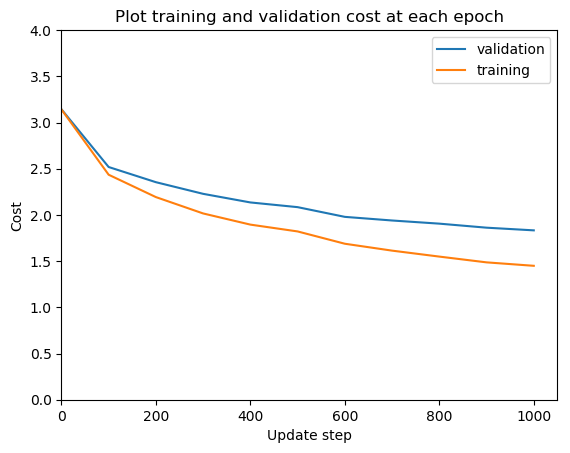
\includegraphics[width=\linewidth]{f3_cost_plt.png}
        \caption{Cost plot}
    \end{subfigure}
    \hfill
    \begin{subfigure}[b]{0.32\textwidth}
        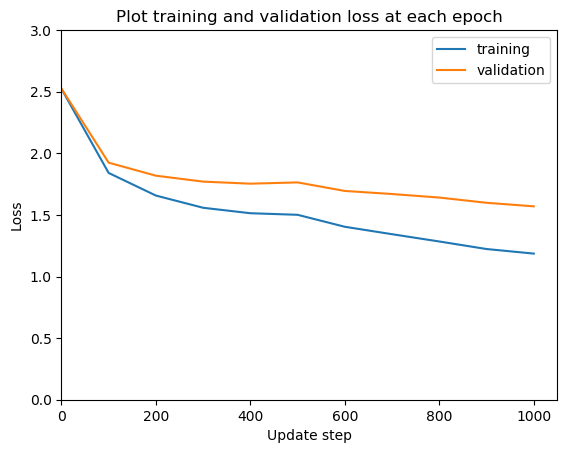
\includegraphics[width=\linewidth]{f3_loss_plt.png}
        \caption{Loss plot}
    \end{subfigure}\hfill
    \begin{subfigure}[b]{0.32\textwidth}%
        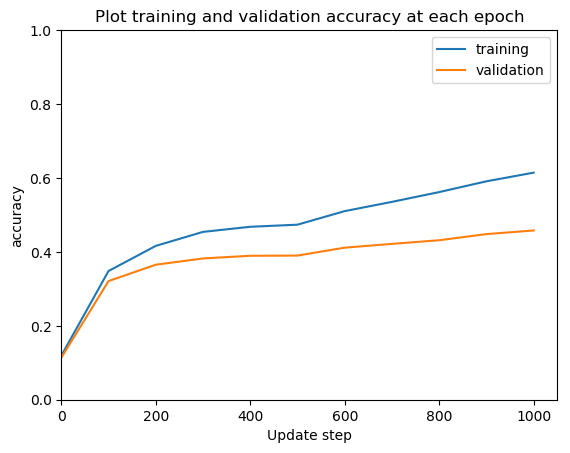
\includegraphics[width=\linewidth]{f3_acc_plt.png}
        \caption{Accuracy plot}
    \end{subfigure}
    \caption{
        Training with default parameters for one cycle:
        \texttt{eta\_min = 1e-5, eta\_max = 1e-1,  lambda = .01 and n\_s = 500}
    }
    \label{fig:replicate_f3}
\end{figure}
\begin{figure}[!htb]
    \begin{subfigure}[b]{0.32\textwidth}
        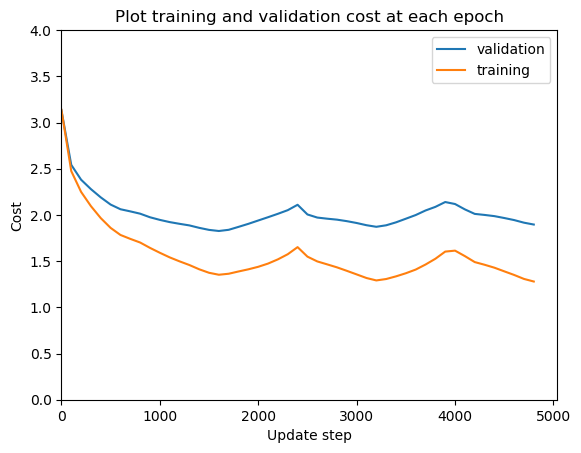
\includegraphics[width=\linewidth]{f4_cost_plt.png}
        \caption{Cost plot}
    \end{subfigure}
    \hfill
    \begin{subfigure}[b]{0.32\textwidth}
        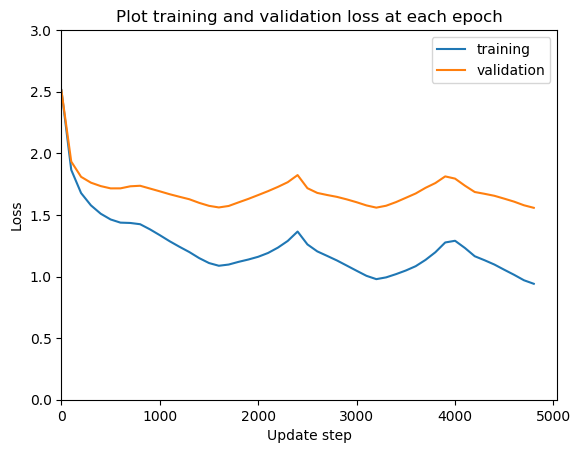
\includegraphics[width=\linewidth]{f4_loss_plt.png}
        \caption{Loss plot}
    \end{subfigure}\hfill
    \begin{subfigure}[b]{0.32\textwidth}%
        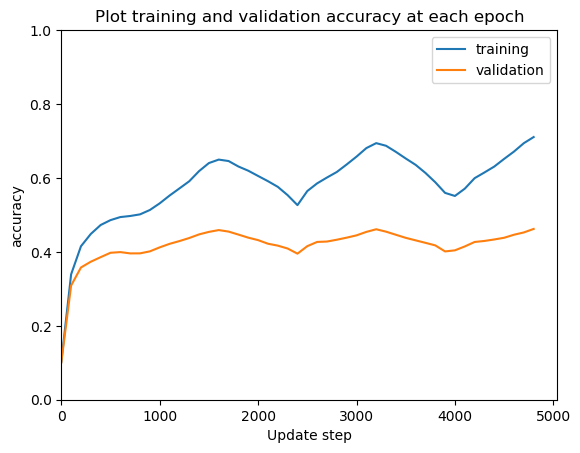
\includegraphics[width=\linewidth]{f4_acc_plt.png}
        \caption{Accuracy plot}
    \end{subfigure}
    \caption{
        Training with default parameters for three cycle:
        \texttt{eta\_min = 1e-5, eta\_max = 1e-1,  lambda = .01 and n\_s = 800}
    }
    \label{fig:replicate_f4}
\end{figure}
\end{question}



\end{document}
